\section{Understanding Performance Bugs} 
\label{s:study}
%To the best of our knowledge, there is currently little knowledge about 
%
In this section, we present an empirical study on several known performance bugs in mainstream Markdown compilers
to help understand the characteristics of the performance bugs. % in Markdown compilers.
%

\subsection{Data Collection}
\label{s:study-bug}

\begin{table}[t]
\centering
    \caption{The existing performance bugs included in our study.
    Lang. means the underlying programming language for implementing the Markdown compiler.
    }
\label{table:study-dataset}
\small
%\resizebox{0.47\textwidth}{!}{
\begin{tabular}{lccc}
   \toprule
      Software  & Lang. & \# Bugs & Time Periods \\
    \midrule
    CommonMark-spec & N/A & 13 & 10/26/2014 - 02/17/2020 \\
    cmark & C & 13 & 01/14/2017 - 12/20/2020 \\
    MD4C  & C & 6 & 03/10/2019 - 09/10/2019\\
    commonmark.js  & JS & 9 & 09/28/2017 - 08/13/2019 \\
    markdown-it & JS & 8 & 08/14/2019 - 11/20/2020\\
%    \midrule
%    Total &  & (49) 52 & 10/26/2014 - 12/20/2020\\
   \bottomrule
\end{tabular}
%}
\end{table}

%As shown in \autoref{table:study-dataset}, 
We investigate performance bugs in the CommonMark specification \cite{commonmark-spec}
%
and 4 representative Markdown compilers chosen from the recommended implementations of the specification \cite{commonmark-spec-list}.
%
%
In particular, cmark \cite{cmark} and MD4C \cite{md4c} are two high-performance Markdown compilers written in C;
cmark is ported and extended for GitHub \cite{cmark-gfm}.
%
commonmark.js \cite{commonmarkjs} and markdown-it \cite{markdown-it} are two Node.js packages that are used in both client-side and server-side applications.
%
We do not consider the software that uses Markdown compilers as one of its sub-components/modules (\eg{,} GitLab \cite{gitlab}), because such software usually does not modify the internal workflow of the included compilers.
%its bug characteristics can be revealed in the analysis of the standalone Markdown compilers.
%
%Such software usually does not introduce new bug features concerning the performance bugs in its Markdown compiler components.
%
We limit our manual analysis to only four representative Markdown compilers because the analysis is quite time-consuming.
%
Furthermore, we find that our current software set already allows us to characterize the bugs and extract some general features,
%
which we will present later in this section.
%

In these Markdown compilers, we manually collected 49 distinct performance bugs from their public bug disclosure channels and their GitHub repository issues. % and collect performance bugs.
%
The bug distribution is presented in \autoref{table:study-dataset}.
%
\iffalse
Some bug reports might be duplicates.
%
We remove a duplicate bug from our dataset if it has a similar cause as another one,
%
though it can have a different exploit vector.
%
In summary, we obtained 49 distinct performance bugs by removing 3 duplicates from the ones reported from October 2014 to December 2020.
%
\fi
%
We found all these performance bugs were abusing the CPU resources instead of other resources like memory.
%
This suggests CPU resource exhaustion performance bugs are the dominant type of performance bugs.
%
%
We next characterize the 49 performance bugs and present our findings.

\subsection{Disclosure and Patch Time}
\label{s:study-time}
\begin{figure}[t]
    \centering
    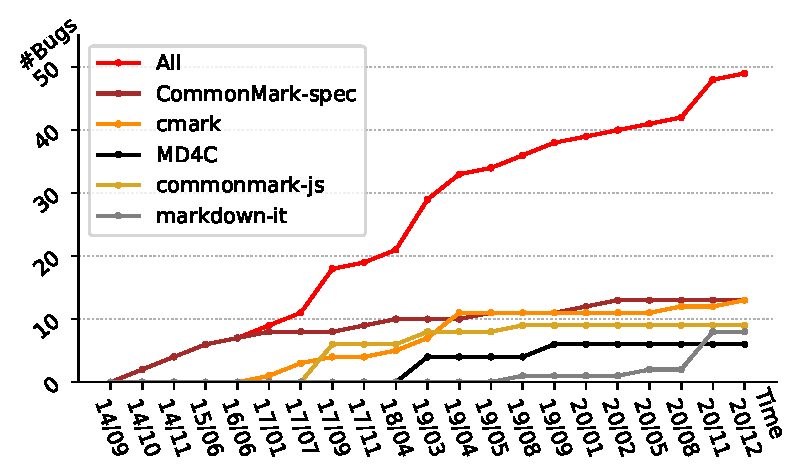
\includegraphics[width=0.45\textwidth, trim =5 0 0 0,clip]{fig/disclosure-time.pdf}
    \caption{The number of performance bug reports over time from October 2014 to December 2020.
    }
    \label{fig:disclosure-time}
\end{figure}

To understand the trend of performance bugs, we analyze the disclosure time of the 49 bugs.
%
We depict the number of performance bugs along the time they were disclosed for each software in \autoref{fig:disclosure-time}.
%
%Unlike other types of bugs such as memory errors \cite{sun2016toward},
%
%we find that performance bugs do not appear throughout the release history of the applications.
%
We observe that few bugs were reported before early 2015, and the number of reported bugs had been gradually growing from early 2018 till late 2020.
%
In particular, 28 (57.14\%) out of the 49 performance bugs were disclosed from April 2018 till December 2020 (22 months);
%
21 (42.86\%) bugs were reported from August 2014 to December 2017 (41 months).
%
It reveals that such bugs had been gradually drawing the attention from the compiler developers and security analysts.
%
%Each individual Markdown compiler also shares a similar bug disclosure trend.
%\WM{<- What does this sentence mean? How is it relevant?}
%\PENGHUI{The figure contains individual software info, but that is not well used yet? I just use the sentence to mention that point}

We further analyze the time it takes to release a patch since a bug is initially reported.
%
We were able to successfully determine the time for 32 performance bugs.
%
For the rest bugs, either we did not find the explicit bug patch time \cite{cmark-218}, or they have not been patched yet \cite{cmark-373}.
%
We find that the average duration to patch performance bugs is 19 days.
%
Further, 23 (71.88\%) bugs were patched within 30 days.
%
We particularly investigated those bugs that took much longer patch time, \eg{}, more than 4 months.
%
We observed that they were usually related to the ambiguity of the CommonMark specification.
%
Thus their patches usually require some work from both the compiler developers and the specification maintainers.
%
Some of the bugs and the patches lead to the modifications of the language specification.


\subsection{Root Causes}
\label{s:study-root-causes}
%There are a large variety of potential causes for performance bugs.
%
Identifying the common root causes of real-world performance bugs can benefit potential future research and software developments.
%
We manually analyzed 49 performance bugs and successfully figured out the root causes for 39 bugs.
%
We classify the root causes into three categories.
%
A bug is assigned to multiple categories if it has multiple major causes.


\PN{R1:} \emph{Super-linear algorithms.}
%crafted inputs that exercise worst-case complexity and exhaust the victim’s computational resources,
Some normal algorithms implemented in Markdown compilers have super-linear worst-case complexity \cite{slowfuzz, perffuzz}.
%although the average complexity is normally linear.
%
Attackers can craft inputs to trigger the worst-case behaviors and lead to performance issues.
%
%For instance, some compilers use regular expressions to match inputs, which are vulnerable to ReDoS attacks \cite{redos} that trigger excessive numbers of backtracking in the matching process.
%
The majority (25 out of 39) of bugs were related to such worst-case behaviors.
%\WM{Check this number again after moving ReDoS to R2.}
%
%Specifically, the abnormal backtracking logic in Markdown compilers can be further divided into two groups:
%
%
%Known performance bugs in this category exploit either the design of Markdown compilers or the vulnerable regular expression and can lead to polynomial or exponential complexity compilation time.
%
%What is worse, the intended normal functionality of the Markdown compilers can be abused by crafted inputs for triggering worst-case behaviors, \eg{,} excessive number of backtracking.
%
%This includes triggering cataphoric backtracking in regular expression matches and the similar logic design inside the Markdown compilers can be abused with specially crafted inputs.
%
%
%If the input size is not limited, the Markdown compilers can easily hang for up to several hours.
%
%
%27 out of 39 performance bugs belong to this category.
%Specially crafted inputs abuse the backtracking behaviors and lead.
%
%We investigate the specially crafted inputs that lead to such worst-case behaviors. %and present two bugs in this category.
%We discuss two primary kinds of algorithms that exhibit the super-linear worst-case complexity we find. % in the Markdown compilers.
%
%They can be roughly divided into two groups:
%
%(1) long open tokens without close tokens,
%
%and (2) long early open tokens and late close tokens.
%

Some Markdown syntaxes (\eg{,} links, emphasis and strong emphasis, HTML blocks) are related to the language's context-sensitive features.
%
%We notice that the performance bugs are quite related to the logic (syntax) of the Markdown language,
%
%in particular, its context-sensitive features.
%
As discussed in \autoref{s:background-compiler},
supporting context-sensitive features in Markdown requires the compilers to backtrack, which could take more than linear time.
%
The backtracking strategies can easily be abused with crafted inputs hence lead to performance issues.
%
%\WM{Check the following. The total number 25+14 are larger than the above 27.}
For instance, links were the primary vulnerable syntax in Markdown compilers,
%
where 11 of the known performance bugs could be exploited with special inputs with links.
%
%Usually, they can happen together with other syntax components.
%
%
%Emphasis and strong emphasis is the second vulnerable Markdown syntax.
%HTML blocks are also the most vulnerable Markdown syntax component in Markdown compilers.
%
Similarly, 8 of the bugs were caused by the buggy emphasis and strong emphasis handlers.
%
Our study reveals that the implementation of the context-sensitive features in the Markdown compilers are prone to containing performance bugs.
%For example, the backtracking from wrong options can be abused and result in performance issues.



One typical input pattern that exploits the context-sensitive syntax handler to trigger performance bugs is \emph{many open tokens}.
%
This pattern can lead the compilers to repeatedly search a close token towards the end of the input string for each such open token, and also force the compilers to backtrack to correct wrong options the compilers have selected.
%
%Regarding the number of repetitions, $n$, the time complexity can be $O(n^2)$ or higher.
%Some logic design of Markdown compilers produces similar backtracking behaviors when a temporal mismatch is detected.
%
For example, deeply nested CDATA block open delimiters can result in an excessive compilation time.
%
%When Markdown compilers detect the first CDATA block open delimiter (\ie{,} \blstinline{<![CDATA[}), they have to search to the end until a matched CDATA block close delimiter (\ie{,} \blstinline{]]>}) is found.
%
%When the match cannot be found, the Markdown compilers perform backtracking to the current CDATA open delimiter.
%
When fed with $n$-nested CDATA block open delimiters (\eg{,} \blstinline{'<![!CDATA[<![CDATA[<![CDATA[...'}) that are not closed with the corresponding close delimiters (\ie{,} \blstinline{']]>'}) or are closed in the end of the input string,
%
%can backtrack repeatedly on every open delimiter and in total for $n$ times.
the compilers need to compare with all tokens in the input string to determine if an open delimiter can be closed or not.
%
Once the compilers find an open delimiter cannot be closed, they switch to other possible options for that delimiter next, for instance, the open delimiter \blstinline{'<!'} in \blstinline{'<!A>'}, which cannot be closed either.
%
%Each time, the compilers have to search till the end of the input string.
%
Thus the time for handling such input strings is at least in polynomial time complexity.
%
By providing a long input with many such open tokens, it is simple to cost the compiler several-second or even more execution time.
%Depending on how such backtracking strategies are designed, such inputs can cause polynomial or higher complexity performance issues, easily resulting in seconds of execution time.


\PN{R2:} \emph{Inefficient code.}
%
Some inefficient code in the Markdown compilers could also lead to performance issues.
%
For instance, some functions do not coordinate well for certain functionalities.
%
We find that 9 performance bugs were caused by such inefficient code.
%
Unlike the algorithms in R1, such performance issues could be addressed by optimizing the inefficient code.
%
However, each problem needs to be separately analyzed and fixed, which could be time-consuming.
%
We next discuss an example of such inefficient code.
%

Minor performance issues in individual problematic functions could accumulate when the given inputs can repeatedly trigger the execution of such functions.
%
For example, in one bug, cmark calls \blstinline{S_find_first_nonspace()} to find the first non-space character from the current offset in a line. %, which has a minor performance issue by
%
%The function went back from the current offset backwardly to find the first non-space character,
The function in a second call would still search from the initial position,
even if in a previous call it has already recognized the location of the first non-space character.
%
This means some function calls to \blstinline{S_find_first_nonspace()} sometimes were unnecessary.
%
Crafted inputs with lots of complicated and nested indents could result in repeated invocations of this function and cause performance bugs.
%
The problem, however, can be solved by using better strategies like cashing the positions of the previously found non-space characters.
%

\iffalse
Second, some Markdown compilers match input strings using regular expressions (regex).
%
Some vulnerable regex could lead to performance bugs if the regex engine needs to backtrack (in exponential time) when matching some specific inputs.
%
A failed matching attempt can lead the engine to backtrack with multiple choices.
%
Thus the total number of possible backtracking paths is exponential if the match cannot be found eventually for every input symbol.
%
This is also known as regular expression denial-of-service (ReDoS) \cite{freezing, shen2018rescue, redosimpact, wustholz2017static}.
%
For instance, one bug in commonmark.js was caused by using a regex containing a vulnerable subexpression \blstinline{(.|\\\\)*]}\footnote{The vulnerable subexpression is simplified for demonstration.}
to match link labels (\eg{}, the \blstinline{[demo]} in \blstinline{'[demo](url 'title')'}).
%
Its syntax is to match any non empty character \blstinline{.} or a single blackslash \blstinline{\\\\} for any number of times \blstinline{*}, followed by a closing bracket \blstinline{]}.
%
%
Suppose the compiler uses this regex to match an input string \blstinline{'\\\\\\\\...'} that contains $n$ backslash characters.
%
The matching would eventually fail because the input string does not contain any closing bracket.
%
But before the failure, the regex engine would check all possible matches for the previous part \blstinline{(.|\\\\)*}.
%
%
Each backslash character in the input string can match either \blstinline{.} or \blstinline{\\\\}, so $n$ characters would cause the engine to backtrack with $2^n$ possible paths.
%
Nevertheless, such performance bugs could be addressed by fixing the vulnerable regex.
\fi
%

\PN{R3:} \emph{Implementation-specific issues.}
Other causes of the bugs are specific to the compiler implementations or designs.
%
Some compilers overlooked part of the CommonMark specification, for example, Unicode support.
%
This can lead to infinite loops when unexpected inputs are provided to the compilers.
%
Some other bugs in this category were caused by wrong data structures.
%
5 performance bugs fall into this category.

\begin{comment}
\subsection{Markdown Syntax and Performance Bugs}
\label{s:study-markdown}

\begin{table}[t]
\caption{Top 4 types of vulnerable Markdown syntax}
\label{tab:bug-syntax}
\centering
\small
\resizebox{0.47\textwidth}{!}{
\begin{tabular}{lcll}
    \toprule
    Markdown syntax & Bugs & Examples  & Root causes\\
    \midrule
    Links & 25 & \blstinline{'[ (]( [ (]( ...'} & \textbf{R1} \textbf{R2} \textbf{R3} \\
    (Strong) Emphasis &14 & \blstinline{'a\_ a\_ ...'} & \textbf{R1} \textbf{R3}\\
    HTML blocks & 9 & \blstinline{'<!\[CDATA\[ <![CDATA[...'} & \textbf{R1} \\
    Fenced code blocks & 5 & \blstinline{'```\\ncode\\n...'} & \textbf{R1}\\
   \bottomrule
\end{tabular}
}
\end{table}

%

We investigate the relationship between the Markdown syntax and the compiler performance bugs.
%
We present the top 4 types of vulnerable Markdown syntaxes of the known performance bugs in \autoref{tab:bug-syntax}.
%
A bug is classified into one or multiple syntax groups if it is caused by the inefficient or incorrect implementations of the syntax(es).
%
%A bug can be classified into several syntax groups if it breaks several syntax handlers.
%
We also list an example for each syntax group in the third column of \autoref{tab:bug-syntax}.
%


We also show the main root causes in each syntax component in the last column of \autoref{tab:bug-syntax}.
%
We include the root cause for a syntax group if at least one bug in the group has that root cause.
%
The results show that unlimited backtracking behaviors were quite common---all the top 4 buggy Markdown syntax components contained bugs with such a root cause.
\WM{<- Check this backtracking.}

\end{comment}


\subsection{Patches of Performance Bugs}
\label{s:study-patch}
We investigate the patches of performance bugs in Markdown compilers to understand how they were addressed.
%
We manage to identify the bug fix patterns for 28 performance bugs.
%
We present our findings below.
%

\PN{P1:} \emph{Enforcing limits.}
%
The most common patch pattern is to add limits for certain conditions such as the maximum depth of the nested structure,
%
although the CommonMark specification does not explicitly specify any such limits.
%
%
When such limits are reached, the compilers directly regard the rest unanalyzed inputs as plain text.
%
%Most uses of Markdown compilers normally do not exceed such limits,
%
%\eg{}, the depth of nested parenthesis seldom reaches thousands of layers.
%
Enforcing limits can prevent excessive CPU usages caused by the worst-case exploitation of too large test cases.
%By adding a limit,
%
However, 
the intended functionality might be violated.
%
It is also difficult to set a correct limit to prevent all attacks while not breaking some unusual yet legitimate inputs.
%the Markdown compilers will abort the tasks and process other tasks if a certain limit is reached.
%
%Such a strategy is simple yet useful.
%
Such a strategy has been applied to patch 13 out of the 28 bugs we investigate.

\PN{P2:} \emph{Logic changes.}
Logic changes sometimes are necessary as the bugs are caused by the incorrect coordination among multiple program components and functions.
%
Some inefficient code snippets need to be further optimized to eliminate the underlying performance issues.
%
For some other performance bugs caused by incorrect regular expressions,
compiler developers mainly review and rewrite the regular expressions.
